\chapter{\ifproject%
\ifenglish Experimentation and Results\else การทดลองและผลลัพธ์\fi
\else%
\ifenglish System Evaluation\else การประเมินระบบ\fi
\fi}

\section{ผลการทดลองที่ 1: การฝึกสอนด้วยชุดข้อมูลดั้งเดิม (Baseline Training with Old Dataset)}
ในการทดลองเบื้องต้น ผู้วิจัยได้ใช้ชุดข้อมูลดั้งเดิม (Old Dataset) เพื่อสร้างค่ามาตรฐานอ้างอิง (Baseline) สำหรับการประเมินประสิทธิภาพของโมเดล โดยได้แยกการวัดผลออกเป็นกรณีภาพถ่ายที่ไม่มีรอยโรคและกรณีภาพถ่ายที่มีรอยโรค

\subsection{ผลลัพธ์สำหรับภาพถ่ายช่องปากที่ไม่มีรอยโรค (Negative Cases)}
สำหรับการทดสอบกับกลุ่มภาพถ่ายที่ไม่ปรากฏรอยโรค ผลการทดสอบเชิงปริมาณแยกตามรายคลาสสำหรับการทดลองที่ 1 แสดงดังตารางที่ \ref{tab:eval_baseline_old_dataset_negative}

\begin{table}[H]
\centering
\caption{ผลการทดสอบเชิงปริมาณของการทดลองที่ 1 สำหรับภาพถ่ายช่องปากที่ไม่มีรอยโรค (Negative Cases)}
\label{tab:eval_baseline_old_dataset_negative}
\begin{tabular}{|l|c|c|c|c|c|}
\hline
\textbf{Class Name} & \textbf{Precision} & \textbf{Recall} & \textbf{F1} & \textbf{IoU} & \textbf{Boundary F1} \\ \hline
Dorsal Tongue & 0.943447 & 0.906059 & 0.924375 & 0.859384 & 0.732060 \\
Tooth & 0.912334 & 0.930648 & 0.921400 & 0.854256 & 0.723160 \\
Buccal Mucosa and Inner Lip & 0.910358 & 0.853435 & 0.880978 & 0.787275 & 0.546532 \\
Outer Lips & 0.861291 & 0.898228 & 0.879372 & 0.784713 & 0.617752 \\
Hard Palate & 0.808795 & 0.601482 & 0.689901 & 0.526602 & 0.853610 \\
Ventral Tongue & 0.795992 & 0.873557 & 0.832973 & 0.713756 & 0.846921 \\
Other Oral Soft Tissues & 0.816171 & 0.733434 & 0.772594 & 0.629453 & 0.705731 \\
Gingiva & 0.742736 & 0.765840 & 0.754111 & 0.605280 & 0.644568 \\ \hline
\textbf{Mean} & \textbf{0.848891} & \textbf{0.820336} & \textbf{0.831963} & \textbf{0.720090} & \textbf{0.708792} \\ \hline
\end{tabular}
\end{table}

\subsection{ผลลัพธ์สำหรับภาพถ่ายช่องปากที่มีรอยโรค (Positive Cases)}
สำหรับการทดสอบกับกลุ่มภาพถ่ายที่ปรากฏรอยโรค เพื่อประเมินความสามารถในการระบุตำแหน่งเนื้อเยื่อปกติท่ามกลางรอยโรคที่เกิดขึ้น ผลการทดสอบเชิงปริมาณสำหรับการทดลองที่ 1 แสดงดังตารางที่ \ref{tab:eval_baseline_old_dataset_positive}

\begin{table}[H]
\centering
\caption{ผลการทดสอบเชิงปริมาณของการทดลองที่ 1 สำหรับภาพถ่ายช่องปากที่มีรอยโรค (Positive Cases)}
\label{tab:eval_baseline_old_dataset_positive}
\begin{tabular}{|l|c|c|c|c|c|}
\hline
\textbf{Class Name} & \textbf{Precision} & \textbf{Recall} & \textbf{F1} & \textbf{IoU} & \textbf{Boundary F1} \\ \hline
Tooth & 0.899780 & 0.920017 & 0.909786 & 0.834502 & 0.667318 \\
Dorsal Tongue & 0.896344 & 0.914619 & 0.905389 & 0.827133 & 0.548999 \\
Buccal Mucosa and Inner Lip & 0.826323 & 0.852368 & 0.839143 & 0.722866 & 0.493512 \\
Gingiva & 0.913975 & 0.735552 & 0.815114 & 0.687926 & 0.392773 \\
Ventral Tongue & 0.888296 & 0.630614 & 0.737597 & 0.584280 & 0.466121 \\
Outer Lips & 0.715442 & 0.720604 & 0.718014 & 0.560079 & 0.724725 \\
Other Oral Soft Tissues & 0.728289 & 0.577558 & 0.644224 & 0.475170 & 0.824469 \\
Hard Palate & 0.564206 & 0.679497 & 0.616508 & 0.445617 & 0.740124 \\ \hline
\textbf{Mean} & \textbf{0.798154} & \textbf{0.752700} & \textbf{0.770697} & \textbf{0.641361} & \textbf{0.607255} \\ \hline
\end{tabular}
\end{table}

ในบทนี้จะเป็นการนำเสนอผลการทดลองและประเมินประสิทธิภาพของตัวแบบในแต่ละขั้นตอนตามที่ได้วางแผนไว้ในบทที่ 3 โดยจะเริ่มจากการวิเคราะห์ผลลัพธ์เชิงปริมาณ (Quantitative Results) ของการทดลองที่มีความสำคัญ

\section{ผลการทดลองที่ 2: การฝึกสอนด้วยชุดข้อมูลฉบับปรับปรุง (New Dataset)}
ในการทดลองนี้ ผู้วิจัยได้ใช้ชุดข้อมูลที่ผ่านการทำความสะอาดและปรับปรุงค่า Ground Truth ใหม่ทั้งหมด เพื่อทดสอบประสิทธิภาพของโมเดล DeepLabV3-resnet50 โดยได้แยกการวัดผลออกเป็นสองกรณีหลัก ได้แก่ กรณีภาพถ่ายที่ไม่มีรอยโรค และกรณีภาพถ่ายที่มีรอยโรค

\subsection{ผลลัพธ์สำหรับภาพถ่ายช่องปากที่ไม่มีรอยโรค (Negative Cases)}
สำหรับการทดสอบกับกลุ่มภาพถ่ายที่ไม่ปรากฏรอยโรค เพื่อประเมินความแม่นยำในการระบุตำแหน่งเนื้อเยื่อปกติในช่องปาก ผลการทดสอบเชิงปริมาณแยกตามรายคลาส (Class-wise Performance) แสดงดังตารางที่ \ref{tab:eval_new_dataset_negative}

\begin{table}[H]
\centering
\caption{ผลการทดสอบเชิงปริมาณของการทดลองที่ 2 สำหรับภาพถ่ายช่องปากที่ไม่มีรอยโรค (Negative Cases)}
\label{tab:eval_new_dataset_negative}
\begin{tabular}{|l|c|c|c|c|c|}
\hline
\textbf{Class Name} & \textbf{Precision} & \textbf{Recall} & \textbf{F1} & \textbf{IoU} & \textbf{Boundary F1} \\ \hline
Buccal Mucosa & 0.90886 & 0.907816 & 0.908337 & 0.832068 & 0.580507 \\
Dorsal Tongue & 0.959935 & 0.913742 & 0.936269 & 0.880175 & 0.780366 \\
Gingiva & 0.781735 & 0.778412 & 0.78007 & 0.639438 & 0.591059 \\
Hard Palate & 0.822469 & 0.818582 & 0.820521 & 0.695663 & 0.85335 \\
Other Soft Tissues & 0.776051 & 0.861055 & 0.816346 & 0.689683 & 0.728003 \\
Outer Lips & 0.895358 & 0.885319 & 0.89031 & 0.802306 & 0.554171 \\
Tooth & 0.932223 & 0.916961 & 0.924529 & 0.859651 & 0.806164 \\
Ventral Tongue & 0.886172 & 0.929118 & 0.907137 & 0.830055 & 0.821613 \\ \hline
\textbf{Mean} & \textbf{0.882568} & \textbf{0.888277} & \textbf{0.885046} & \textbf{0.799275} & \textbf{0.71408} \\ \hline
\end{tabular}
\end{table}

\subsection{ผลลัพธ์สำหรับภาพถ่ายช่องปากที่มีรอยโรค (Positive Cases)}
สำหรับการทดสอบกับกลุ่มภาพถ่ายที่ปรากฏรอยโรค เพื่อประเมินความสามารถในการระบุตำแหน่งเนื้อเยื่อปกติท่ามกลางรอยโรคที่เกิดขึ้น ผลการทดสอบเชิงปริมาณแยกตามรายคลาสแสดงดังตารางที่ \ref{tab:eval_new_dataset_positive}

\begin{table}[H]
\centering
\caption{ผลการทดสอบเชิงปริมาณของการทดลองที่ 2 สำหรับภาพถ่ายช่องปากที่มีรอยโรค (Positive Cases)}
\label{tab:eval_new_dataset_positive}
\begin{tabular}{|l|c|c|c|c|c|}
\hline
\textbf{Class Name} & \textbf{Precision} & \textbf{Recall} & \textbf{F1} & \textbf{IoU} & \textbf{Boundary F1} \\ \hline
Buccal Mucosa & 0.885269 & 0.86346 & 0.874228	& 0.776559 & 0.437987 \\
Dorsal Tongue & 0.954927 & 0.928354 & 0.941453 & 0.889383 & 0.594855 \\
Gingiva & 0.730454 & 0.787679 & 0.757988	& 0.610291 & 0.48934 \\
Hard Palate & 0.879042 & 0.775759 & 0.824178 & 0.700937 & 0.786896 \\
Other Soft Tissues & 0.857824 & 0.742822 & 0.796192 & 0.661394 & 0.687714 \\
Outer Lips & 0.913906 & 0.802013 & 0.854312 & 0.745675 & 0.52605 \\
Tooth & 0.945897 & 0.944894 & 0.945395 & 0.896445 & 0.706354 \\
Ventral Tongue & 0.844425 & 0.870158 & 0.857098 & 0.749932 & 0.798505 \\ \hline
\textbf{Mean} & \textbf{0.881555} & \textbf{0.84915} & \textbf{0.863952} & \textbf{0.765622} & \textbf{0.628462} \\ \hline
\end{tabular}
\end{table}


\section{ผลการทดลองที่ 3: การประยุกต์ใช้เทคนิคการเตรียมข้อมูลภาพ (New Dataset + Preprocessing)}
ในการทดลองนี้ ผู้วิจัยได้นำชุดข้อมูลฉบับปรับปรุงจากการทดลองที่ 2 มาผ่านกระบวนการเตรียมข้อมูลภาพ (Image Preprocessing) เพื่อปรับปรุงคุณภาพของลักษณะเด่นให้ชัดเจนยิ่งขึ้น โดยผลลัพธ์ในส่วนของภาพถ่ายที่ไม่มีรอยโรคแสดงดังตารางที่ \ref{tab:eval_preprocessing_negative}

\subsection{ผลลัพธ์สำหรับภาพถ่ายช่องปากที่ไม่มีรอยโรค (Negative Cases)}
ผลการทดสอบเชิงปริมาณแยกตามรายคลาสสำหรับการทดลองที่ 3 ในกรณีที่ไม่ปรากฏรอยโรค แสดงได้ดังนี้:

\begin{table}[H]
\centering
\caption{ผลการทดสอบเชิงปริมาณของการทดลองที่ 3 สำหรับภาพถ่ายช่องปากที่ไม่มีรอยโรค (Negative Cases)}
\label{tab:eval_preprocessing_negative}
\begin{tabular}{|l|c|c|c|c|c|}
\hline
\textbf{Class Name} & \textbf{Precision} & \textbf{Recall} & \textbf{F1} & \textbf{IoU} & \textbf{Boundary F1} \\ \hline
Buccal Mucosa & 0.90714 & 0.906194 & 0.906666 & 0.829268 & 0.60803 \\
Dorsal Tongue & 0.951201 & 0.918155 & 0.934386 & 0.876852 & 0.792895 \\
Gingiva & 0.803239 & 0.754522 & 0.778119 & 0.636821 & 0.614153 \\
Hard Palate & 0.893199 & 0.903508 & 0.898324 & 0.815416 & 0.834026 \\
Other Soft Tissues & 0.796122 & 0.862291 & 0.827886 & 0.706319 & 0.710024 \\
Outer Lips & 0.957176 & 0.869626 & 0.911303 & 0.837059 & 0.672034 \\
Tooth & 0.950972 & 0.92634 & 0.938494 & 0.884116 & 0.812111 \\
Ventral Tongue & 0.871275 & 0.926401 & 0.897993 & 0.81487 & 0.847207 \\ \hline
\textbf{Mean} & \textbf{0.900933} & \textbf{0.89466} & \textbf{0.897183} & \textbf{0.81826} & \textbf{0.73631} \\ \hline
\end{tabular}
\end{table}

\subsection{ผลลัพธ์สำหรับภาพถ่ายช่องปากที่มีรอยโรค (Positive Cases)}
สำหรับการทดสอบกับกลุ่มภาพถ่ายที่มีรอยโรคเพื่อประเมินประสิทธิภาพภายใต้เงื่อนไขที่มีความซับซ้อนของพื้นที่รอยโรค ผลการทดสอบเชิงปริมาณสำหรับการทดลองที่ 3 แสดงดังตารางที่ \ref{tab:eval_preprocessing_positive}

\begin{table}[H]
\centering
\caption{ผลการทดสอบเชิงปริมาณของการทดลองที่ 3 สำหรับภาพถ่ายช่องปากที่มีรอยโรค (Positive Cases)}
\label{tab:eval_preprocessing_positive}
\begin{tabular}{|l|c|c|c|c|c|}
\hline
\textbf{Class Name} & \textbf{Precision} & \textbf{Recall} & \textbf{F1} & \textbf{IoU} & \textbf{Boundary F1} \\ \hline
Buccal Mucosa & 0.853986 & 0.862108 & 0.858028 & 0.751356 & 0.459404 \\
Dorsal Tongue & 0.93859 & 0.911461 & 0.924826 & 0.860165 & 0.593017 \\
Gingiva & 0.770775 & 0.782912 & 0.776796 & 0.635051 & 0.508513 \\
Hard Palate & 0.908998 & 0.82505 & 0.864992 & 0.762102 & 0.845697 \\
Other Soft Tissues & 0.860266 & 0.808275 & 0.83346 & 0.714472 & 0.679746 \\
Outer Lips & 0.903241 & 0.795517 & 0.845964 & 0.733047 & 0.514259 \\
Tooth & 0.961615 & 0.950146 & 0.955846 & 0.915426 & 0.745578 \\
Ventral Tongue & 0.873055 & 0.870708 & 0.87188 & 0.772861 & 0.758351 \\ \hline
\textbf{Mean} & \textbf{0.888615} & \textbf{0.859845} & \textbf{0.8735} & \textbf{0.779237} & \textbf{0.638071} \\ \hline
\end{tabular}
\end{table}

\section{ผลการทดลองที่ 4: การปรับจูนผลลัพธ์ด้วยกระบวนการตรวจแก้หลังการประมวล (New Dataset + Preprocessing + Postprocessing)}
ในการทดลองขั้นสุดท้าย ผู้วิจัยได้นำผลลัพธ์ที่ผ่านกระบวนการเตรียมข้อมูลภาพและการฝึกสอนด้วยชุดข้อมูลฉบับปรับปรุง มาผ่านกระบวนการตรวจแก้หลังการประมวล (Post-processing) เพื่อกำจัดสัญญาณรบกวนและปรับปรุงความสมบูรณ์ของพื้นที่พยากรณ์ โดยผลลัพธ์สำหรับภาพถ่ายที่ไม่มีรอยโรคแสดงดังตารางที่ \ref{tab:eval_postprocessing_negative}

\subsection{ผลลัพธ์สำหรับภาพถ่ายช่องปากที่ไม่มีรอยโรค (Negative Cases)}
ผลการทดสอบเชิงปริมาณสำหรับการทดลองที่ 4 ในกรณีที่ไม่ปรากฏรอยโรค แสดงได้ดังนี้:

\begin{table}[H]
\centering
\caption{ผลการทดสอบเชิงปริมาณของการทดลองที่ 4 สำหรับภาพถ่ายช่องปากที่ไม่มีรอยโรค (Negative Cases)}
\label{tab:eval_postprocessing_negative}
\begin{tabular}{|l|c|c|c|c|c|}
\hline
\textbf{Class Name} & \textbf{Precision} & \textbf{Recall} & \textbf{F1} & \textbf{IoU} & \textbf{Boundary F1} \\ \hline
Buccal Mucosa & 0.904933 & 0.915577 & 0.910224 & 0.835239 & 0.619343 \\
Dorsal Tongue & 0.962795 & 0.933173 & 0.947753 & 0.900694 & 0.79416 \\
Gingiva & 0.804554 & 0.775137 & 0.789572 & 0.652308 & 0.625187 \\
Hard Palate & 0.898375 & 0.904478 & 0.901416 & 0.820525 & 0.840006 \\
Other Soft Tissues & 0.822041 & 0.856972 & 0.839143 & 0.722865 & 0.714018 \\
Outer Lips & 0.958763 & 0.877711 & 0.916449 & 0.845782 & 0.694432 \\
Tooth & 0.950796 & 0.929097 & 0.939822 & 0.886475 & 0.808706 \\
Ventral Tongue & 0.893669 & 0.923479 & 0.908329 & 0.832054 & 0.851051 \\ \hline
\textbf{Mean} & \textbf{0.908475} & \textbf{0.899882} & \textbf{0.903837} & \textbf{0.828917} & \textbf{0.743878} \\ \hline
\end{tabular}
\end{table}

\subsection{ผลลัพธ์สำหรับภาพถ่ายช่องปากที่มีรอยโรค (Positive Cases)}
สำหรับการทดสอบกับกลุ่มภาพถ่ายที่มีรอยโรค เพื่อประเมินประสิทธิภาพของกระบวนการ Post-processing ภายใต้ความซับซ้อนของรอยโรค ผลการทดสอบเชิงปริมาณแยกตามรายคลาสสำหรับการทดลองที่ 4 แสดงได้ดังนี้:

\begin{table}[H]
\centering
\caption{ผลการทดสอบเชิงปริมาณของการทดลองที่ 4 สำหรับภาพถ่ายช่องปากที่มีรอยโรค (Positive Cases)}
\label{tab:eval_postprocessing_positive}
\begin{tabular}{|l|c|c|c|c|c|}
\hline
\textbf{Class Name} & \textbf{Precision} & \textbf{Recall} & \textbf{F1} & \textbf{IoU} & \textbf{Boundary F1} \\ \hline
Buccal Mucosa & 0.854437 & 0.861782 & 0.858094 & 0.751457 & 0.473734 \\
Dorsal Tongue & 0.9397 & 0.911545 & 0.925409 & 0.861172 & 0.635301 \\
Gingiva & 0.773713 & 0.778721 & 0.776209 & 0.634266 & 0.561558 \\
Hard Palate & 0.915219 & 0.826638 & 0.868676 & 0.767841 & 0.857924 \\
Other Soft Tissues & 0.863066 & 0.807518 & 0.834369 & 0.715808 & 0.769126 \\
Outer Lips & 0.903279 & 0.795434 & 0.845933 & 0.733002 & 0.527017 \\
Tooth & 0.95384 & 0.955339 & 0.954589 & 0.913123 & 0.739635 \\
Ventral Tongue & 0.875597 & 0.870852 & 0.873218 & 0.774966 & 0.771889 \\ \hline
\textbf{Mean} & \textbf{0.889551} & \textbf{0.860035} & \textbf{0.874032} & \textbf{0.780047} & \textbf{0.771889} \\ \hline
\end{tabular}
\end{table}

\section{สรุปผลการศึกษาตามลำดับขั้นตอน (Ablation Study Summary)}
เพื่อให้เห็นพัฒนาการและประสิทธิภาพที่เพิ่มขึ้นในแต่ละขั้นตอนของงานวิจัย ผู้วิจัยได้นำค่าเฉลี่ย (Mean) ของตัวชี้วัดความแม่นยำจากทั้ง 4 การทดลองหลักมาทำการเปรียบเทียบแบบเคียงข้างกัน (Side-by-side Comparison) เพื่อวิเคราะห์ผลกระทบของกระบวนการปรับปรุงข้อมูล การเตรียมภาพ และการตรวจแก้หลังการประมวล โดยสรุปได้ดังตารางที่ \ref{tab:ablation_negative_summary} และ \ref{tab:ablation_positive_summary}

\begin{table}[H]
\centering
\caption{สรุปการเปรียบเทียบค่าเฉลี่ยสำหรับการทดสอบกับภาพถ่ายช่องปากที่ไม่มีรอยโรค (Negative Cases)}
\label{tab:ablation_negative_summary}
\begin{tabular}{|l|c|c|c|c|c|}
\hline
\textbf{การทดลอง (Experiments)} & \textbf{Precision} & \textbf{Recall} & \textbf{F1} & \textbf{IoU} & \textbf{Boundary F1} \\ \hline
1: Baseline (Old Dataset) & 0.848891 & 0.820336 & 0.831963 & 0.720090 & 0.708792 \\
2: New Dataset & 0.882568 & 0.888277 & 0.885046 & 0.799275 & 0.714080 \\
3: New Dataset + Preprocessing & 0.900933 & 0.894660 & 0.897183 & 0.818260 & 0.736310 \\
4: Final (New + Pre + Post) & \textbf{0.908475} & \textbf{0.899882} & \textbf{0.903837} & \textbf{0.828917} & \textbf{0.743878} \\ \hline
\end{tabular}
\end{table}

\begin{table}[H]
\centering
\caption{สรุปการเปรียบเทียบค่าเฉลี่ยสำหรับการทดสอบกับภาพถ่ายช่องปากที่มีรอยโรค (Positive Cases)}
\label{tab:ablation_positive_summary}
\begin{tabular}{|l|c|c|c|c|c|}
\hline
\textbf{การทดลอง (Experiments)} & \textbf{Precision} & \textbf{Recall} & \textbf{F1} & \textbf{IoU} & \textbf{Boundary F1} \\ \hline
1: Baseline (Old Dataset) & 0.798154 & 0.752700 & 0.770697 & 0.641361 & 0.607255 \\
2: New Dataset & 0.881555 & 0.849150 & 0.863952 & 0.765622 & 0.628462 \\
3: New Dataset + Preprocessing & 0.888615 & 0.859845 & 0.873500 & 0.779237 & 0.638071 \\
4: Final (New + Pre + Post) & \textbf{0.889551} & \textbf{0.860035} & \textbf{0.874032} & \textbf{0.780047} & \textbf{0.771889} \\ \hline
\end{tabular}
\end{table}

\section{วิเคราะห์ผลการทดลองและการอภิปราย (Discussion)}
จากการเปรียบเทียบผลการทดลองทั้ง 4 ขั้นตอน พบข้อสังเกตและประเด็นสำคัญที่สะท้อนถึงประสิทธิภาพของระบบดังนี้:

\begin{enumerate}
    \item \textbf{ผลของการปรับปรุงชุดข้อมูล (Dataset Improvement):} เมื่อเปรียบเทียบจากการทดลองที่ 1 ไปยังการทดลองที่ 2 พบว่าค่าตัวชี้วัด F1-Score และ IoU เพิ่มขึ้นอย่างก้าวกระโดด (โดยเฉพาะในกรณี Positive Cases ที่ F1 เพิ่มจาก 0.77 เป็น 0.86) สิ่งนี้แสดงให้เห็นว่าความถูกต้องของผลเฉลย (Ground Truth Labels) มีผลอย่างยิ่งต่อการเรียนรู้ของโมเดล การทำความสะอาดข้อมูลทำให้โมเดลสับสนระหว่างเนื้อเยื่อปกติและรอยโรคน้อยลง
    \item \textbf{ผลของเทคนิคการเตรียมภาพ (Preprocessing Effect):} การเพิ่มขั้นตอนการเตรียมภาพในการทดลองที่ 3 ช่วยยกระดับค่าความแม่นยำขึ้นอย่างต่อเนื่อง โดยเฉพาะค่า Boundary F1 และ IoU ที่เพิ่มสูงขึ้น แสดงให้เห็นว่าการปรับปรุงลักษณะเด่นทางภาพทัศน์ช่วยให้โมเดลสามารถระบุขอบเขตของเนื้อเยื่อต่างๆ ได้ชัดเจนยิ่งขึ้นแม้ในสภาพแสงหรือสีผิวภาพถ่ายที่แตกต่างกัน
    \item \textbf{ประสิทธิภาพของกระบวนการหลังการประมวล (Post-processing):} ในการทดลองที่ 4 กระบวนการตรวจแก้ภายหลังจากได้ผลลัพธ์จากโมเดลช่วยกำจัดสัญญาณรบกวน (Noise Removal) และเติมเต็มพื้นที่ส่วนพยากรณ์ให้มีความสมบูรณ์มากขึ้น ส่งผลให้ค่า Boundary F1 ในกรณี Positive Cases เพิ่มขึ้นอย่างมีนัยสำคัญ (จาก 0.63 สู่ 0.77) ซึ่งช่วยให้ผลการแบ่งส่วนมีลักษณะที่เรียบเนียนและสอดคล้องกับโครงสร้างจริงทางกายวิภาคศาสตร์มากที่สุด
\end{enumerate}

\section{วิเคราะห์ข้อผิดพลาดและข้อจำกัด (Error Analysis \& Limitations)}
แม้ตัวแบบขั้นสุดท้ายจะแสดงประสิทธิภาพที่น่าพึงพอใจในระดับภาพรวม แต่จากการตรวจสอบผลลัพธ์ในระดับพิกเซล ผู้วิจัยยังพบข้อผิดพลาดบางประการและข้อจำกัดที่ท้าทายสำหรับการนำไปใช้งานจริง ดังนี้:

\begin{enumerate}
    \item \textbf{ความยากในการแบ่งส่วนเนื้อเยื่อหรือรอยโรคที่มีขนาดเล็ก (Small Object Detection):} โดยเฉพาะในคลาสที่มีอัตราส่วนเนื้อเยื่อน้อยมากเมื่อเทียบกับพื้นที่ทั้งหมด (เช่น Hard Palate และพื้นที่รอยโรคในช่วงเริ่มต้น) โมเดลมักจะพยากรณ์ขอบเขตได้ไม่ครอบคลุมเท่าที่ควร เนื่องจากข้อจำกัดของฟังก์ชัน Dice Loss ที่อาจให้ความสำคัญกับเนื้อเยื่อโครงสร้างหลักมากกว่าพื้นที่ขนาดเล็กเกินไป
    \item \textbf{ความผิดพลาดจากการสับสนระหว่างคลาสที่มีลักษณะกายภาพคล้ายกัน (Inter-class Ambiguity):} ในสภาวะแสงที่ไม่คงที่หรือภาพที่มีค่าสีใกล้เคียงกัน พบว่ามีการพยากรณ์ขอบเขตที่สับสนระหว่างเหงือก (Gingiva) และพิกัดขอบเขตของกระพุ้งแก้ม (Buccal Mucosa) ซึ่งส่งผลให้ค่า Precision ของคลาสเหล่านี้ลดลงในบางกรณี
    \item \textbf{อิทธิพลของปัจจัยทางกายภาพภายนอก (External Factors):} สัญญาณรบกวนในภาพถ่ายช่องปาก เช่น แสงสะท้อนจากความชื้น (Specularity from saliva), ความมืดจากการบดบังด้วยมุมกล้อง และความเบลอจากการเคลื่อนไหว (Motion Blur) ยังคงเป็นอุปสรรคสำคัญที่ทำให้ตัวแบบพยากรณ์ขอบเขตได้คลาดเคลื่อน แม้จะมีการทำ Image Preprocessing แล้วก็ตาม
\end{enumerate}

\section{ผลการทดลองเชิงคุณภาพ (Qualitative Results)}
นอกเหนือจากการประเมินเชิงปริมาณด้วยตัวเลข ผู้วิจัยได้ทำการเลือกตัวอย่างภาพถ่ายจากชุดทดสอบเพื่อแสดงผลลัพธ์การแบ่งส่วนพื้นที่เนื้อเยื่อ (Segmentation Masks) เปรียบเทียบผลลัพธ์ที่ได้จากโมเดลขั้นสุดท้าย ดังแสดงในรูปที่ \ref{fig:qualitative_results}

\begin{figure}[H]
    \centering
    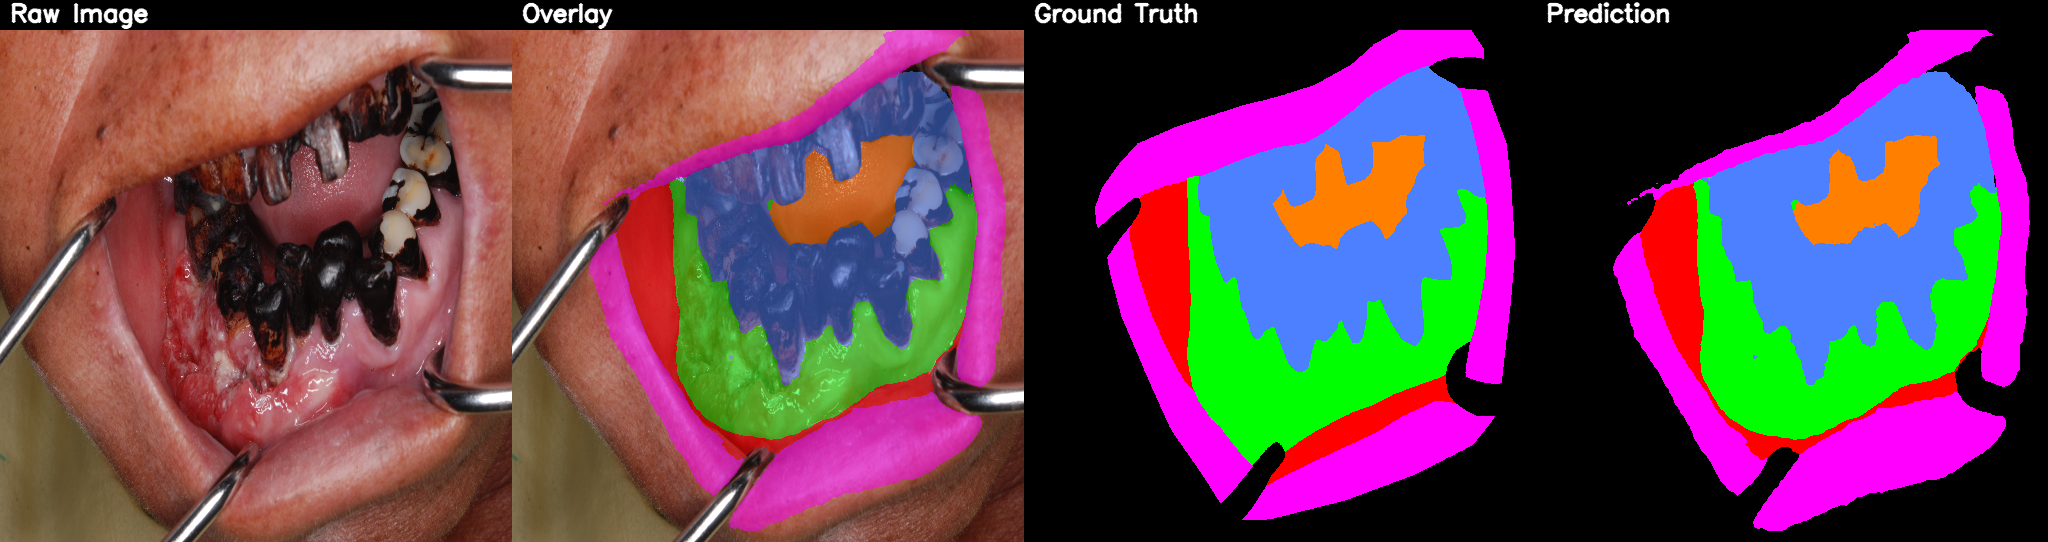
\includegraphics[width=0.7\textwidth]{imge-Inhun/DSC_0137(1).png} \\
    \small (ก) ตัวอย่างภาพที่ 1 \\[2ex]
    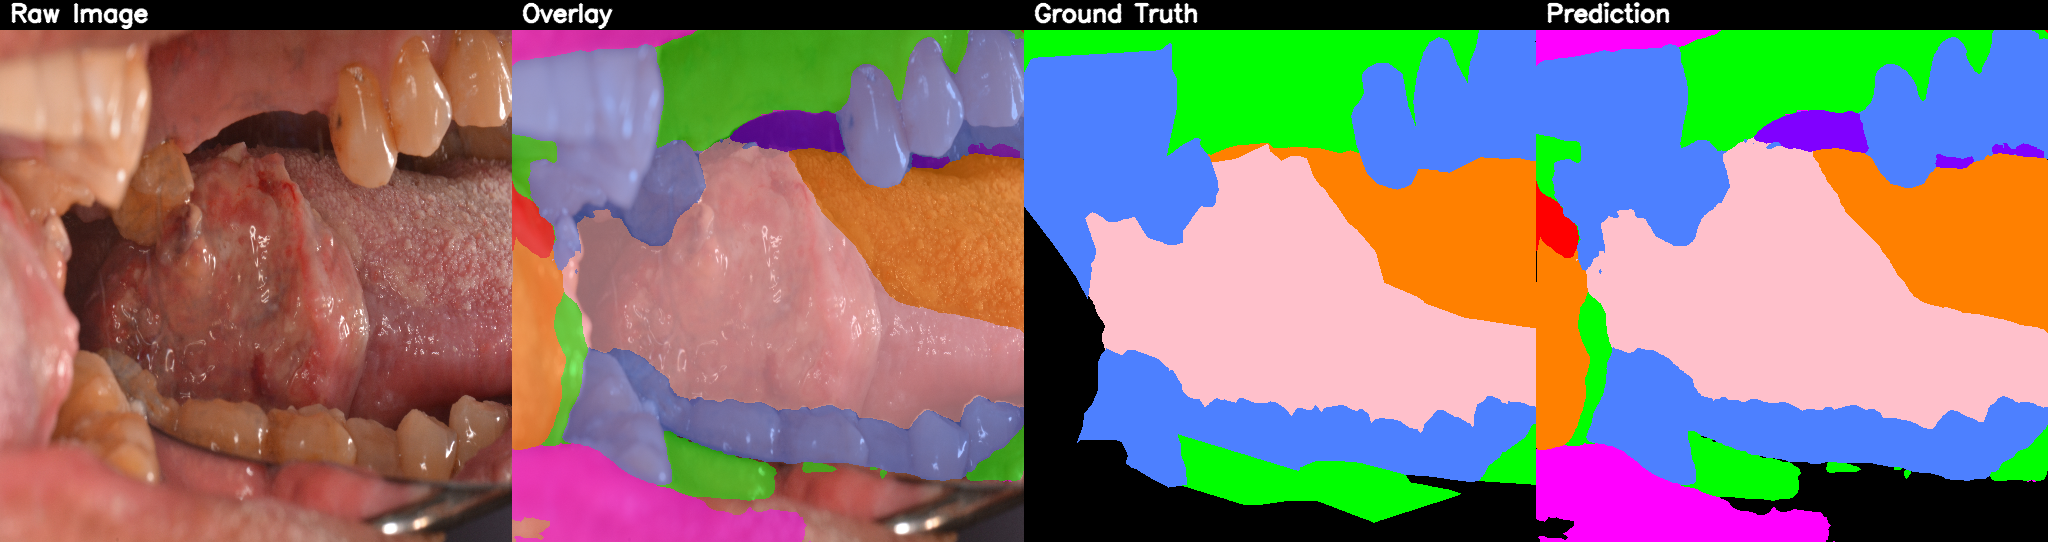
\includegraphics[width=0.7\textwidth]{imge-Inhun/DSC_00450.png} \\
    \small (ข) ตัวอย่างภาพที่ 2 \\[2ex]
    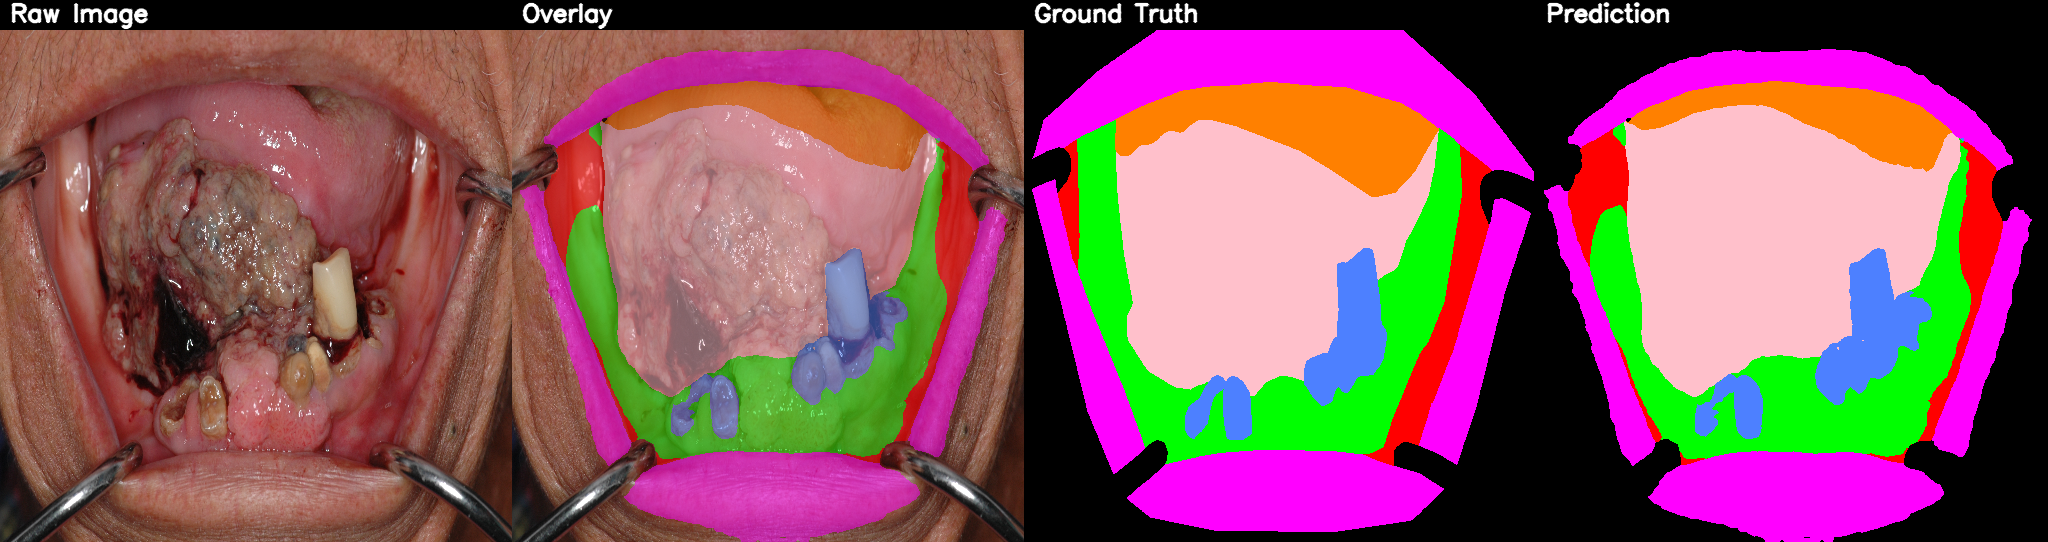
\includegraphics[width=0.7\textwidth]{imge-Inhun/DSC_7929.png} \\
    \small (ค) ตัวอย่างภาพที่ 3
    \caption{การแสดงผลลัพธ์การแบ่งส่วนพื้นที่เนื้อเยื่อจากโมเดลขั้นสุดท้าย (Final Model)}
    \label{fig:qualitative_results}
\end{figure}

จากภาพตัวอย่างทั้ง 3 กรณี จะเห็นได้ว่าโมเดลขั้นสุดท้ายสามารถระบุขอบเขตของเนื้อเยื่อเป้าหมายได้อย่างแม่นยำและมีความต่อเนื่องของพื้นที่ แม้ในสภาพแสงและมุมกล้องที่แตกต่างกัน โดยผลลัพธ์ที่ได้มีลักษณะขอบที่เรียบเนียนซึ่งเป็นผลมาจากกระบวนการจัดเตรียมภาพและการตรวจแก้หลังการประมวลผลที่เหมาะสม

